%%%
% Plantilla de Memoria
% Modificación de una plantilla de Latex de Nicolas Diaz para adaptarla 
% al castellano y a las necesidades de escribir informática y matemáticas.
%
% Editada por: Mario Román
%
% License:
% CC BY-NC-SA 3.0 (http://creativecommons.org/licenses/by-nc-sa/3.0/)
%%%

%%%%%%%%%%%%%%%%%%%%%%%%%%%%%%%%%%%%%%%%%
% Thin Sectioned Essay
% LaTeX Template
% Version 1.0 (3/8/13)
%
% This template has been downloaded from:
% http://www.LaTeXTemplates.com
%
% Original Author:
% Nicolas Diaz (nsdiaz@uc.cl) with extensive modifications by:
% Vel (vel@latextemplates.com)
%
% License:
% CC BY-NC-SA 3.0 (http://creativecommons.org/licenses/by-nc-sa/3.0/)
%
%%%%%%%%%%%%%%%%%%%%%%%%%%%%%%%%%%%%%%%%%

%----------------------------------------------------------------------------------------
%	PAQUETES Y CONFIGURACIÓN DEL DOCUMENTO
%----------------------------------------------------------------------------------------

%%% Configuración del papel.
% microtype: Tipografía.
% mathpazo: Usa la fuente Palatino.
\documentclass[a4paper, 20pt]{article}
\usepackage[a4paper,margin=1in]{geometry}
\usepackage[protrusion=true,expansion=true]{microtype}
\usepackage{mathpazo}

% Indentación de párrafos para Palatino
\setlength{\parindent}{0pt}
  \parskip=8pt
\linespread{1.05} % Change line spacing here, Palatino benefits from a slight increase by default


%%% Castellano.
% noquoting: Permite uso de comillas no españolas.
% lcroman: Permite la enumeración con numerales romanos en minúscula.
% fontenc: Usa la fuente completa para que pueda copiarse correctamente del pdf.
\usepackage[spanish,es-noquoting,es-lcroman,es-tabla,,es-nodecimaldot]{babel}
\usepackage[utf8]{inputenc}
\usepackage{fontenc}
\selectlanguage{spanish}


%%% Gráficos
\usepackage{graphicx} % Required for including pictures
\usepackage{wrapfig} % Allows in-line images
\usepackage[usenames,dvipsnames]{color} % Coloring code
%\usepackage{subcaption}
\usepackage{subfig}
\graphicspath{{./fig/}}


%%% Matemáticas
\usepackage{amsmath}
\usepackage{physics} % para las derivadas parciales
\usepackage[Symbol]{upgreek} %pi

%%% Pseudocódigo
\usepackage{algorithmicx}
\usepackage[ruled]{algorithm}
\usepackage{algpseudocode}

\newcommand{\alg}{\texttt{algorithmicx}}
\newcommand{\old}{\texttt{algorithmic}}
\newcommand{\euk}{Euclid}
\newcommand\ASTART{\bigskip\noindent\begin{minipage}[b]{0.5\linewidth}}
\newcommand\ACONTINUE{\end{minipage}\begin{minipage}[b]{0.5\linewidth}}
\newcommand\AENDSKIP{\end{minipage}\bigskip}
\newcommand\AEND{\end{minipage}}

%%% Código
\usepackage{listings}

%%% Tablas
\usepackage{tabularx}
\usepackage{float}
\usepackage{adjustbox}
\usepackage{booktabs}

% Enlaces y colores
\usepackage{hyperref}
\usepackage[dvipsnames]{xcolor}
\definecolor{webgreen}{rgb}{0,0.5,0}
\hypersetup{
  colorlinks=true,
  citecolor=RoyalBlue,
  urlcolor=RoyalBlue,
  linkcolor=RoyalBlue
}

%%% Bibliografía
\usepackage[backend=biber]{biblatex}
\DefineBibliographyStrings{spanish}{
  urlseen = {Último acceso}
}
\addbibresource{IN-P2.bib}


%%% Subsubsection con letras
\renewcommand{\thesubsubsection}{\thesubsection.\alph{subsubsection}}

%%% Itemize, enumitem
\usepackage{paralist}
\usepackage{enumitem}
%----------------------------------------------------------------------------------------
%	TÍTULO
%----------------------------------------------------------------------------------------
% Configuraciones para el título.
% El título no debe editarse aquí.
\renewcommand{\maketitle}{
  \begin{flushright} % Right align
  
  {\LARGE\@title} % Increase the font size of the title
  
  \vspace{50pt} % Some vertical space between the title and author name
  
  {\large\@author} % Author name
  \\\@date % Date
  \vspace{40pt} % Some vertical space between the author block and abstract
  \end{flushright}
}

%% Título
\title{\textbf{Título}\\ % Title
Subtítulo} % Subtitle

\author{\textsc{Autor1,\\Autor2} % Author
\\{\textit{Universidad de Granada}}} % Institution

\date{\today} % Date

%-----------------------------------------------------------------------------------------
%	DOCUMENTO
%-----------------------------------------------------------------------------------------

\begin{document}

%-----------------------------------------------------------------------------------------
%	TITLE PAGE
%-----------------------------------------------------------------------------------------

\begin{titlepage} % Suppresses displaying the page number on the title page and the subsequent page counts as page 1
	
	\raggedleft % Right align the title page
	
	\rule{1pt}{\textheight} % Vertical line
	\hspace{0.05\textwidth} % Whitespace between the vertical line and title page text
	\parbox[b]{0.8\textwidth}{ % Paragraph box for holding the title page text, adjust the width to move the title page left or right on the page
		
		{\Huge\bfseries Trabajo 2:\\[0.5\baselineskip] Programación\\[2\baselineskip]} % Title
		{\large\textit{Curso 2019/2020}\\[0.5\baselineskip]Aprendizaje Automático\\[1\baselineskip] }% Subtitle or further description
		{\Large\textsc{Sofía Almeida Bruno}\\[0.5\baselineskip]sofialmeida@correo.ugr.es} % Author name, lower case for consistent small caps
		
		\vspace{0.4\textheight} % Whitespace between the title block and the publisher
		
		{\noindent \\[0.5\baselineskip] }\\[\baselineskip] % Publisher and logo
	}

\end{titlepage}

%% Resumen (Descomentar para usarlo)
%\renewcommand{\abstractname}{Resumen} % Uncomment to change the name of the abstract to something else
%\begin{abstract}
% Resumen aquí
%\end{abstract}

%% Palabras clave
%\hspace*{3,6mm}\textit{Keywords:} lorem , ipsum , dolor , sit amet , lectus % Keywords
%\vspace{30pt} % Some vertical space between the abstract and first section


%% Índice
{\parskip=2pt
  \tableofcontents
}
\pagebreak

%%% Inicio del documento
%%%%%%%%%%%%%%%%%%%%%%%%%%%%%%%%%%%%%%%%%%%%%%%%%%%%%%%%%%%%%%%%%%%
%       EJERCICIO 1
%%%%%%%%%%%%%%%%%%%%%%%%%%%%%%%%%%%%%%%%%%%%%%%%%%%%%%%%%%%%%%%%%%%
\large
\section{Ejercicio sobre la búsqueda complejidad de H y el ruido}
El código correspondiente a este ejercicio se encuentra en el archivo \texttt{ej1.py}.
\subsection{Dibujar una gráfica con la nube de puntos de salida correspondiente.}
Para dibujar las gráficas con la nube de puntos se ha implementado la función \texttt{draw\_points} que toma como parámetro el vector $N$ de puntos.
\subsubsection{Considere $N = 50$, $dim = 2$, $rango = [-50, +50]$ con \texttt{simula\_unif(N, dim, rango)}.}
Llamando a la función \texttt{simula\_unif(N, dim, rango)} con los parámetros correspondintes, se generó el conjunto de puntos que podemos observar en la Figura \ref{fig:1a}. Notamos que, efectivamente, los puntos se han generado uniformemente en el rango.

\begin{figure}[H]
    \centering
    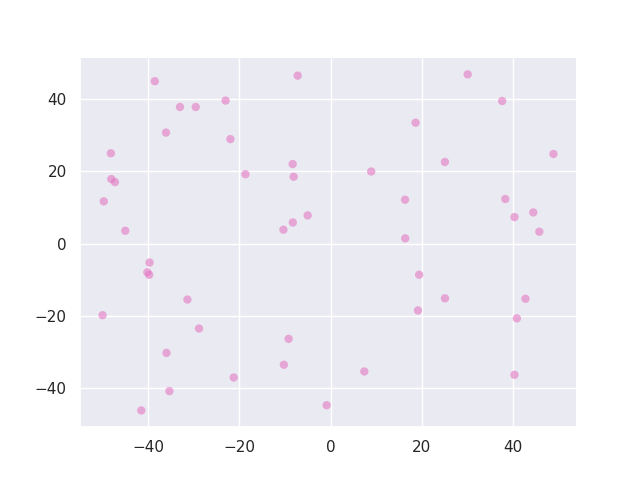
\includegraphics[width=0.75\textwidth]{points1a}
    \caption{Puntos generados con \texttt{simula\_unif}.}
    \label{fig:1a}
\end{figure}

\subsubsection{Considere $N = 50$ y $sigma = [5,7]$ con \texttt{simula\_gaus(N, dim, sigma)}.}
Ejecutando la función \texttt{simula\_gaus} con los parámetros pedidos se obtiene el conjunto de puntos mostrado en la Figura \ref{fig:1b}. En este caso los puntos se agrupan en torno al $(0,0)$ ya que la función usada para generarlos fue una gaussiana de media 0.

\begin{figure}[H]
    \centering
    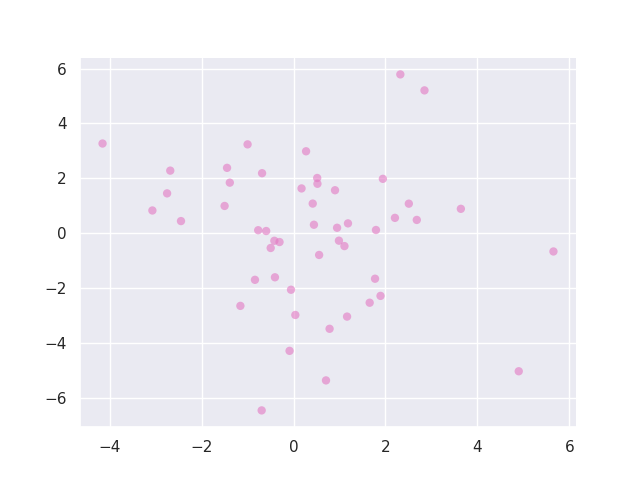
\includegraphics[width=0.75\textwidth]{points1b}
    \caption{Puntos generados con \texttt{simula\_gaus}.}
    \label{fig:1b}
\end{figure}

\subsection{Vamos a valorar la influencia del rudio en la seleccion de la complejidad de la clase de funciones. Con ayuda de la función \texttt{simula\_unif(100, 2, [-50,50])} generar una muestra de puntos 2D a los que vamos añadir una etiqueta usando el signo de la función $f(x, y) = y - ax - b$, es decir el signo de la distancia de cada punto a la recta simulada con \texttt{simula\_recta()}.}
\subsubsection{Dibujar una gráfica donde los puntos muestren el resultado de su etiqueta, junto con la recta usada para ello. (Observe que todos los puntos están bien clasificados respecto de la recta).}

Se generan los puntos como en el caso anterior, en este caso tomamos una muestra de 100 puntos en el mismo rango. Se les asigna su clase mediante la función \texttt{f}, que toma los parámetros \texttt{a, b} obtenidos al ejecutar \texttt{simula\_recta}. Se ha utilizado la función \texttt{plot\_line} para generar la gráfica.

\begin{figure}[H]
    \centering
    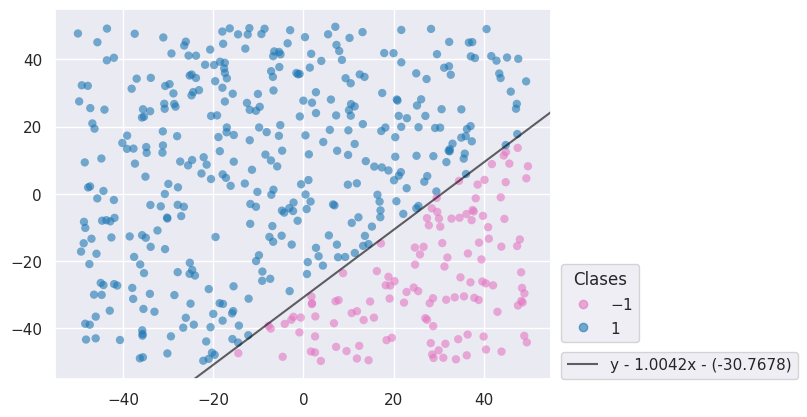
\includegraphics[width=0.75\textwidth]{recta}
    \caption{Puntos generados con \texttt{simula\_unif}, clase asignada a partir del signo de la recta.}
    \label{fig:recta}
\end{figure}

En la Figura \ref{fig:recta} vemos los puntos generados coloreados según su clase y notamos cómo la recta es una frontera perfecta entre ambas. Esto es debido a que las etiquetas se asignaron en función al signo\footnote{De aquí en adelante se considerará que signo(0) = 1 a la hora de asignar las clases.} obtenido por la función que define la recta.

\subsubsection{Modifique de forma aleatoria un 10 \% etiquetas positivas y otro 10 \% de negativas y guarde los puntos con sus nuevas etiquetas. Dibuje de nuevo la gráfica anterior. (Ahora hay puntos mal clasificados respecto de la recta).}

En la función \texttt{modify\_classes} modificamos un 10\% de las etiquetas positivas y un 10\% de las etiquetas negativas. Pintamos la gráfica resultante, que podemos ver en la Figura \ref{fig:2b}. La gráfica es similar a la del apartado anterior, con la diferencia de que esta vez la recta no serpara correctamente a todos los puntos, al haber añadido ruido hay puntos que quedan mal clasificados.

\begin{figure}[H]
    \centering
    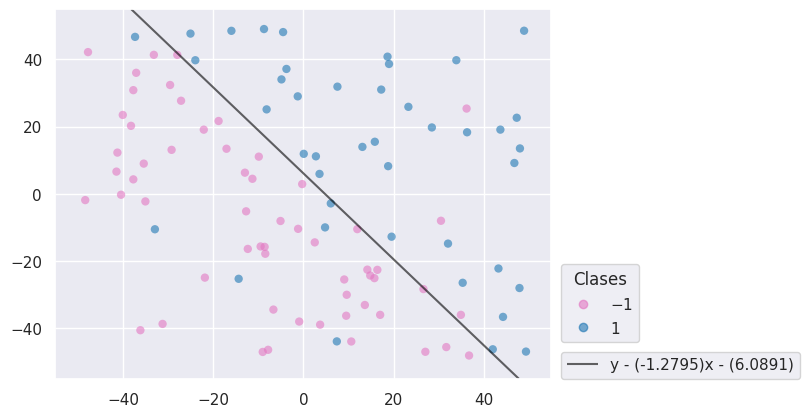
\includegraphics[width=0.75\textwidth]{recta+ruido}
    \caption{Puntos generados con \texttt{simula\_unif}, clase asignada a partir del signo de la recta y posterior adición de ruido al 10\% de las etiquetas de cada clase.}
    \label{fig:2b}
\end{figure}

\subsection{Supongamos ahora que las siguientes funciones definen la frontera de clasificación de los puntos de la muestra en lugar de una recta:}\linespread{-10}
\textbf{
  \begin{itemize}[]
  \item $f_1 (x, y) = (x - 10)^2 + (y - 20)^2 - 400$
  \item $f_2 (x, y) = 0,5(x + 10)^2 + (y - 20)^2 - 400$
  \item $f_3 (x, y) = 0,5(x - 10)^2 - (y + 20)^2 - 400$
  \item $f_4 (x, y) = y - 20x^2 - 5x + 3$
  \end{itemize}
  Visualizar el etiquetado generado en 2b junto con cada una de las gráficas de cada una de las funciones. Comparar las regiones positivas y negativas de estas nuevas funciones con las obtenidas en el caso de la recta. ¿Son estas funciones más complejas mejores clasificadores que la función lineal? Observe las gráficas y diga que consecuencias extrae sobre la influencia del proceso de modificación de etiquetas en el proceso de aprendizaje Explicar el razonamiento.}

La Figura \ref{f:13} muestra las fronteras de clasificación al usar las funciones dadas en el enunciado para definirlas, para generarlas se usó la función \texttt{plot}. A simple vista no parece que las nuevas funciones se ajusten correctamente a las clases dadas. La función $f_1$ clasifica la mayor parte de los puntos como -1, cuando realmente pertenecen a ambas clases, y solo un pequeño grupo como 1, estos, exceptuando los puntos ruidosos, están bien clasificados. Los puntos de la clase -1 quedan, salvo ruido, bien clasificados. La función $f_2$ es parecida a $f_1$ aunque en este caso la elipse es mayor y ahora recoge a puntos de las dos clases (aproximadamente la mitad de ellos quedarán mal clasificados), al resto de puntos se les asigna clase -1, clasificando correctamente aproximadamente la mitad de los puntos. Las funciones $f_3$ y $f_4$, al contrario, asignan a la mayor parte de los puntos la etiqueta 1. En el caso de $f_4$ es más exagerado, dejando con clase 1 a puntos que eran de la clase contraria prácticamente en su totalidad, aunque casi todos los puntos de la clase 1 sí que tienen su clase correcta. La función $f_3$ genera unas regiones en las que asignará clase -1, una de ellas (la derecha) asigna incorrectamente etiqueta -1 a puntos de la clase 1. La otra región en que asigna clase -1 (la izquierda) está formada, en su mayoría, por puntos de esta clase.

\begin{figure}[H]
\def\tabularxcolumn#1{m{#1}}
\begin{tabularx}{\linewidth}{@{}cXX@{}}
%
\begin{tabular}{cc}
\subfloat[$f_1 (x, y) = (x - 10)^2 + (y - 20)^2 - 400$.]{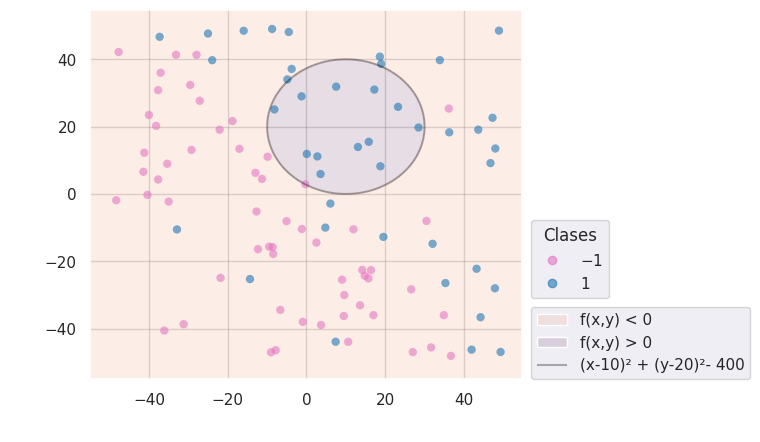
\includegraphics[width=0.5\textwidth]{f1}} 
   & \subfloat[$f_2 (x, y) = 0,5(x + 10)^2 + (y - 20)^2 - 400$.]{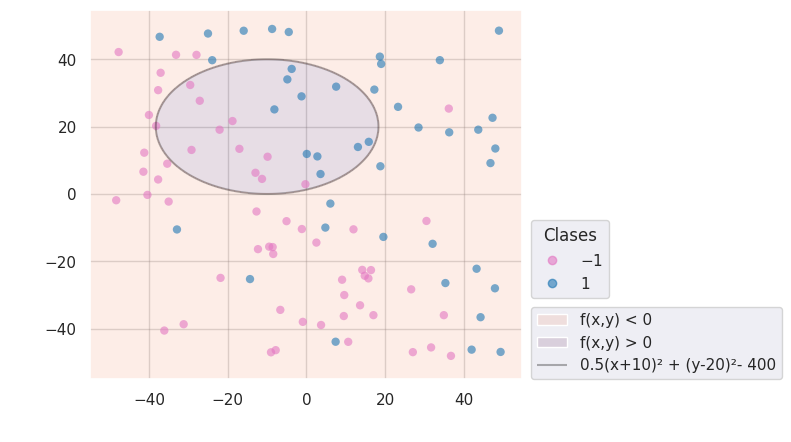
\includegraphics[width=0.5\textwidth]{f2}}\\
\subfloat[$f_3 (x, y) = 0,5(x - 10)^2 - (y + 20)^2 - 400$.]{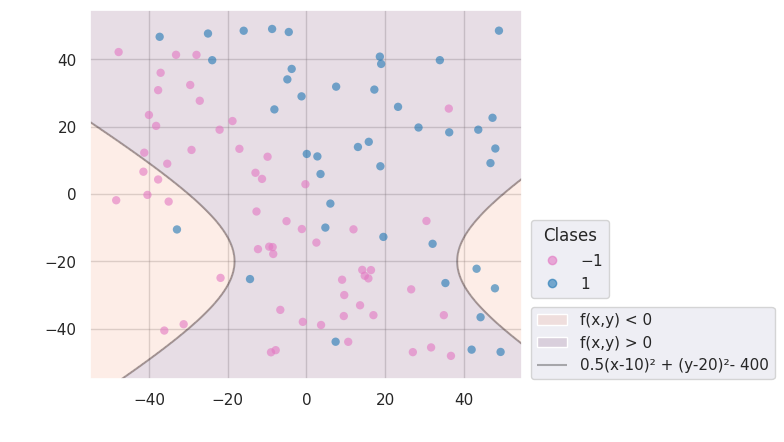
\includegraphics[width=0.5\textwidth]{f3}} 
   & \subfloat[$f_4 (x, y) = y - 20x^2 - 5x + 3$.]{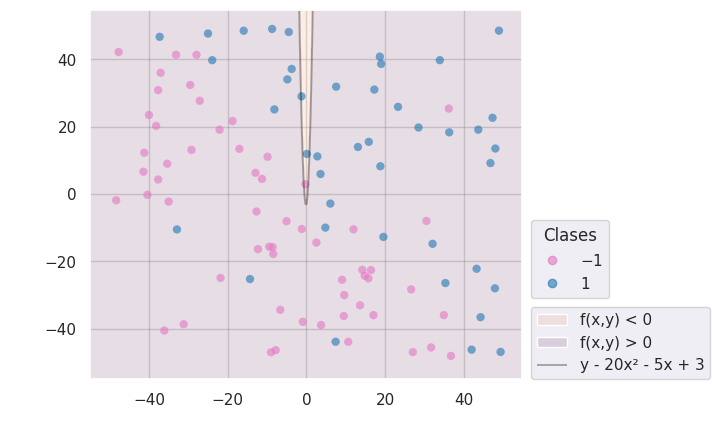
\includegraphics[width=0.5\textwidth]{f4}}\\
\end{tabular}
\end{tabularx}

\caption{Fronteras de clasificación dadas por $f_i$.}\label{f:13}
\end{figure}

A la vista de las gráficas, observamos imprecisión en las clasificaciones dadas por estas regiones, sin embargo, para realizar una comparación más exacta entre ellas podemos hacer uso de alguna métrica. Por un lado, utilizaremós el \textit{accuracy}, que promedia la cantidad de elementos bien clasificados,\[
accuracy = \frac{TP + TN}{P + N},
\]
donde en este caso resulta indiferente qué clase es la positiva y cuál la negativa, ya que no representan nada. El \textit{accuracy} será un valor entre 0 y 1, cuanto más cercano a 1, mejor clasificados estarán los datos.

Como las clases están ligeramente desbalanceadas, hay menos puntos de la clase 1 que de la clase -1, podemos utilizar también una métrica que tenga esto en cuenta, elegimos \textit{balanced accuracy}, esta es una media del \textit{recall} de cada clase. El \textit{recall} viene dado por \[
recall = \frac{TP}{TP+FN},
\]
es una medida de cómo de bien se clasifican los ejemplos positivos, por ello nos interesa promediarlo para ambas clases. También es una medida que se encuentra entre 0 y 1, que cuanto más cercana 1 mejores resultados indica.

En la Tabla \ref{tab:13} se incluyen los valores obtenidos usando las métricas descritas de las funciones de este apartado, además de la función $f(x,y) = y -ax -b$ que determinó en un principio la clase de los puntos.

\begin{table}[H]
\large
\centering
\caption{\textit{Accuracy} y \textit{balanced accuracy} obtenido al clasificar con distintas funciones.}
\label{tab:13}
\begin{tabular}{lrr}
\toprule
& \textit{Accuracy} & \textit{Balanced accuracy}\\ \midrule
$f$ & 0.91 & 0.903\\
$f_1$ & 0.31 & 0.366\\
$f_2$ & 0.43 & 0.476\\
$f_3$ & 0.53 & 0.467\\
$f_4$ & 0.59 & 0.515\\
\bottomrule
\end{tabular}
\end{table}

Como es natural, la función $f$ es la que presenta mejores valores de ambas métricas, no llegan a ser un 1 exacto porque hemos generado un ruido de un 10\% en cada clase, que se corresponde con el 0.1 restante del \textit{accuracy}. Las funciones más complejas $f_i$, como habíamos observado, no separan correctamente las clases fijadas, siendo el mejor \textit{accuracy} de 0.59. En este caso elegir modelos más complejos no ha proporcionado buenos resulados, al contrario que en la práctica anterior.

\section{Modelos lineales}

\subsection{\textbf{Algoritmo Perceptron}: Implementar la función \texttt{ajusta\_PLA(datos, label,\\ max\_iter, vini)} que calcula el hiperplano solución a un problema de clasificación binaria usando el algoritmo PLA. La entrada \texttt{datos} es una matriz donde cada item con su etiqueta está representado por una fila de la matriz, \texttt{label} el vector de etiquetas (cada etiqueta es un valor +1 o -1), \texttt{max\_iter} es el número máximo de iteraciones permitidas y \texttt{vini} el valor inicial del vector. La función devuelve los coeficientes del hiperplano.}

Las funciones implementadas en este apartado, en particular \texttt{ajusta\_PLA}, se encuentran en el archivo \texttt{ej2.py}.

\subsubsection{Ejecutar el algoritmo PLA con los datos simulados en los apartados 2a de la sección.1. Inicializar el algoritmo con: a) el vector cero y, b) con vectores de números aleatorios en [0, 1] (10 veces). Anotar el número medio de iteraciones necesarias en ambos para converger. Valorar el resultado relacionando el punto de inicio con el número de iteraciones.}

En este caso, nos encontramos frente a un conjunto de puntos separable, el algoritmo PLA, aunque necesite muchas iteraciones, encontrará el hiperplano que separa a los conjuntos.

Tomando como punto inicial $w_0 = (0,0,0)^T$, las diez ejecuciones el algoritmo necesita \textbf{315 iteraciones} para encontrar el hiperplano que clasifica correctamente a todos los puntos. En la Figura \ref{fig:21} podemos ver el hiperplano generado por el algoritmo PLA al partir de $w_0$, notamos cómo todos los puntos están bien clasificados. Notamos que el algoritmo es determinista, al empezar en el mismo punto, obtiene los mismos resultados.

\begin{figure}[H]
    \centering
    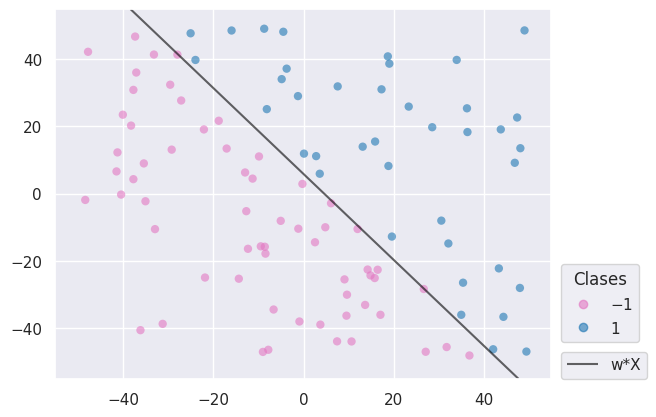
\includegraphics[width=0.75\textwidth]{21}
    \caption{Hiperplano generado por el algoritmo PLA cuando el punto inicial fue $(0,0,0)^T$.}
    \label{fig:21}
\end{figure}

Si tomamos como puntos iniciales vectores aleatorios en $[0,1]$ el número de iteraciones necesarios varía, en el mejor caso necesita 172 iteraciones y en el peor 370. El \textbf{número medio de iteraciones requerido es de 291}, ligeramente inferior al caso anterior, sin embargo la desviación típica es de 61. Destacamos que cada punto inicial requiere un número de iteraciones variable, algunos mejores y otros peores que el caso anterior.

Como ocurre en general, los parámetros de un algoritmo afectan al desempeño del mismo. En este caso hemos observado cómo el punto inicial provoca un aumento o disminución en el número de iteraciones necesario para que el algoritmo encuentre los coeficientes del hiperplano que separa ambas clases. Sin embargo, notamos que, aunque el número de iteraciones varíe según el punto inicial, se logra encontrar el hiperplano que separa correctamente ambas clases, obtemos en todas las ocasiones un \textit{accuracy} de 1.

\subsubsection{Hacer lo mismo que antes usando ahora los datos del apartado 2b de la sección.1. ¿Observa algún comportamiento diferente? En caso afirmativo diga cuál y las razones para que ello ocurra.}

Repetimos la experimentación utilizando el conjunto de datos con ruido. En este caso las clases ya no son separables, los puntos ruidosos se encuentran rodeados por elementos de la clase contraria.

En esta ocasión, el algoritmo alcanza el número máximo de iteraciones sin llegar a conseguir un hiperplano que separe ambas clases. El \textit{accuracy} obtenido varía según el punto inicial, aunque para todos los puntos iniciales es cercano a 0.9, pues solo tenemos un 10\% de error. En la Figura \ref{fig:21ruido} observamos el hiperplano generado cuando el punto inicial fue $(0,0,0)^T$. Notamos como los puntos ruidosos, además de los cercanos a la recta, quedan mal clasificados. 

\begin{figure}[H]
    \centering
    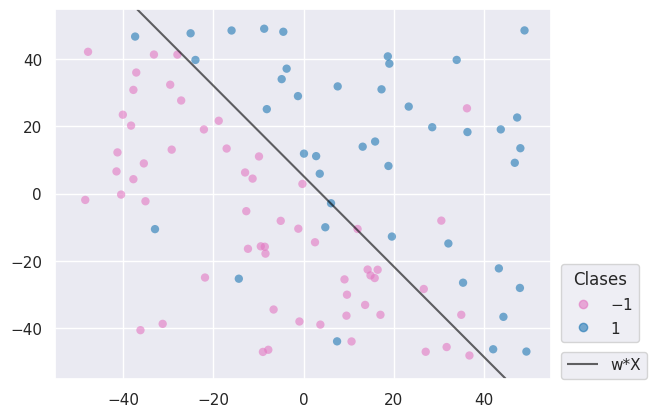
\includegraphics[width=0.75\textwidth]{21ruido}
    \caption{Hiperplano generado por el algoritmo PLA partiendo del punto $(0,0,0)^T$.}
    \label{fig:21ruido}
\end{figure}

\newpage
%%%%%%%%%%%%%%%%%%%%%%%%%%%%%%%%%%%%%%%%%%%%%%%%%%%%%%%%%%%%%%%%%%%
%       REFERENCIAS
%%%%%%%%%%%%%%%%%%%%%%%%%%%%%%%%%%%%%%%%%%%%%%%%%%%%%%%%%%%%%%%%%%%
\printbibliography
\end{document}
